\begin{problem}{1}
\textbf{Visualization}

\begin{figure}[ht!]
	\centering
	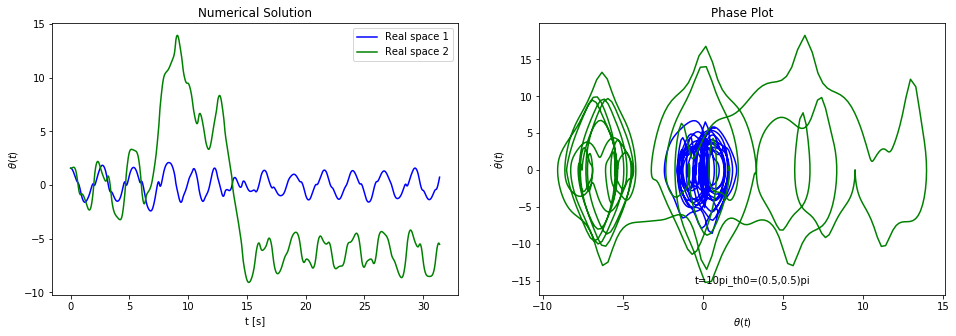
\includegraphics[scale=0.6]{../figures/t=10pi_th0=(05,05)pidoublePend.png}
	\caption{Trajectory of double pendulum}
	\label{double}
\end{figure}

\begin{figure}[ht!]
	\centering
	\includegraphics[scale=0.5]{../figures/.png}
	\caption{Screenshot of double pendulum animation}
	\label{double}
\end{figure}

\end{problem}

\begin{problem}{2}
\textbf{Lyapunov Exponent}

\begin{figure}[ht!]
	\centering
	%\includegraphics[scale=0.6]{../figures/.png}
	\caption{}
	\label{}
\end{figure}

\end{problem}

\begin{problem}{3}
\textbf{Transition to Chaos}

\begin{figure}[ht!]
	\centering
	%\includegraphics[scale=0.6]{../figures/.png}
	\caption{}
	\label{}
\end{figure}

\end{problem}

\begin{problem}{4}
\textbf{Time for First Flip}

\begin{figure}[ht!]
	\centering
	%\includegraphics[scale=0.6]{../figures/.png}
	\caption{}
	\label{}
\end{figure}

\end{problem}